\documentclass[twoside]{book}

% Packages required by doxygen
\usepackage{fixltx2e}
\usepackage{calc}
\usepackage{doxygen}
\usepackage[export]{adjustbox} % also loads graphicx
\usepackage{graphicx}
\usepackage[utf8]{inputenc}
\usepackage{makeidx}
\usepackage{multicol}
\usepackage{multirow}
\PassOptionsToPackage{warn}{textcomp}
\usepackage{textcomp}
\usepackage[nointegrals]{wasysym}
\usepackage[table]{xcolor}

% Font selection
\usepackage[T1]{fontenc}
\usepackage[scaled=.90]{helvet}
\usepackage{courier}
\usepackage{amssymb}
\usepackage{sectsty}
\renewcommand{\familydefault}{\sfdefault}
\allsectionsfont{%
  \fontseries{bc}\selectfont%
  \color{darkgray}%
}
\renewcommand{\DoxyLabelFont}{%
  \fontseries{bc}\selectfont%
  \color{darkgray}%
}
\newcommand{\+}{\discretionary{\mbox{\scriptsize$\hookleftarrow$}}{}{}}

% Page & text layout
\usepackage{geometry}
\geometry{%
  a4paper,%
  top=2.5cm,%
  bottom=2.5cm,%
  left=2.5cm,%
  right=2.5cm%
}
\tolerance=750
\hfuzz=15pt
\hbadness=750
\setlength{\emergencystretch}{15pt}
\setlength{\parindent}{0cm}
\setlength{\parskip}{3ex plus 2ex minus 2ex}
\makeatletter
\renewcommand{\paragraph}{%
  \@startsection{paragraph}{4}{0ex}{-1.0ex}{1.0ex}{%
    \normalfont\normalsize\bfseries\SS@parafont%
  }%
}
\renewcommand{\subparagraph}{%
  \@startsection{subparagraph}{5}{0ex}{-1.0ex}{1.0ex}{%
    \normalfont\normalsize\bfseries\SS@subparafont%
  }%
}
\makeatother

% Headers & footers
\usepackage{fancyhdr}
\pagestyle{fancyplain}
\fancyhead[LE]{\fancyplain{}{\bfseries\thepage}}
\fancyhead[CE]{\fancyplain{}{}}
\fancyhead[RE]{\fancyplain{}{\bfseries\leftmark}}
\fancyhead[LO]{\fancyplain{}{\bfseries\rightmark}}
\fancyhead[CO]{\fancyplain{}{}}
\fancyhead[RO]{\fancyplain{}{\bfseries\thepage}}
\fancyfoot[LE]{\fancyplain{}{}}
\fancyfoot[CE]{\fancyplain{}{}}
\fancyfoot[RE]{\fancyplain{}{\bfseries\scriptsize Generated by Doxygen }}
\fancyfoot[LO]{\fancyplain{}{\bfseries\scriptsize Generated by Doxygen }}
\fancyfoot[CO]{\fancyplain{}{}}
\fancyfoot[RO]{\fancyplain{}{}}
\renewcommand{\footrulewidth}{0.4pt}
\renewcommand{\chaptermark}[1]{%
  \markboth{#1}{}%
}
\renewcommand{\sectionmark}[1]{%
  \markright{\thesection\ #1}%
}

% Indices & bibliography
\usepackage{natbib}
\usepackage[titles]{tocloft}
\setcounter{tocdepth}{3}
\setcounter{secnumdepth}{5}
\makeindex

% Hyperlinks (required, but should be loaded last)
\usepackage{ifpdf}
\ifpdf
  \usepackage[pdftex,pagebackref=true]{hyperref}
\else
  \usepackage[ps2pdf,pagebackref=true]{hyperref}
\fi
\hypersetup{%
  colorlinks=true,%
  linkcolor=blue,%
  citecolor=blue,%
  unicode%
}

% Custom commands
\newcommand{\clearemptydoublepage}{%
  \newpage{\pagestyle{empty}\cleardoublepage}%
}

\usepackage{caption}
\captionsetup{labelsep=space,justification=centering,font={bf},singlelinecheck=off,skip=4pt,position=top}

%===== C O N T E N T S =====

\begin{document}

% Titlepage & ToC
\hypersetup{pageanchor=false,
             bookmarksnumbered=true,
             pdfencoding=unicode
            }
\pagenumbering{alph}
\begin{titlepage}
\vspace*{7cm}
\begin{center}%
{\Large Chess }\\
\vspace*{1cm}
{\large Generated by Doxygen 1.8.14}\\
\end{center}
\end{titlepage}
\clearemptydoublepage
\pagenumbering{roman}
\tableofcontents
\clearemptydoublepage
\pagenumbering{arabic}
\hypersetup{pageanchor=true}

%--- Begin generated contents ---
\chapter{Chess}
\label{md__r_e_a_d_m_e}
\Hypertarget{md__r_e_a_d_m_e}
Personal project to play around with C++ and AI. Supported on both mac\+OS, Windows and Linux. Uses the S\+F\+ML library for the graphic interface. The goal for this personal project is twofold\+:
\begin{DoxyEnumerate}
\item To gain a better understanding of c++ and how to use it in it\textquotesingle{}s full potential.
\item To challenge myself in creating an as-\/smart-\/as-\/possible AI that can beat all my chess-\/rivals!
\end{DoxyEnumerate}

 
\chapter{Hierarchical Index}
\section{Class Hierarchy}
This inheritance list is sorted roughly, but not completely, alphabetically\+:\begin{DoxyCompactList}
\item \contentsline{section}{Board}{\pageref{class_board}}{}
\item \contentsline{section}{Chess\+Piece}{\pageref{class_chess_piece}}{}
\begin{DoxyCompactList}
\item \contentsline{section}{Bishop}{\pageref{class_bishop}}{}
\item \contentsline{section}{King}{\pageref{class_king}}{}
\item \contentsline{section}{Knight}{\pageref{class_knight}}{}
\item \contentsline{section}{Pawn}{\pageref{class_pawn}}{}
\item \contentsline{section}{Queen}{\pageref{class_queen}}{}
\item \contentsline{section}{Rook}{\pageref{class_rook}}{}
\end{DoxyCompactList}
\item \contentsline{section}{Interface}{\pageref{class_interface}}{}
\item \contentsline{section}{Move}{\pageref{class_move}}{}
\item \contentsline{section}{Player}{\pageref{class_player}}{}
\begin{DoxyCompactList}
\item \contentsline{section}{Human\+Player}{\pageref{class_human_player}}{}
\item \contentsline{section}{Min\+Max\+Player}{\pageref{class_min_max_player}}{}
\item \contentsline{section}{Random\+Player}{\pageref{class_random_player}}{}
\end{DoxyCompactList}
\item \contentsline{section}{Square}{\pageref{class_square}}{}
\end{DoxyCompactList}

\chapter{Class Index}
\section{Class List}
Here are the classes, structs, unions and interfaces with brief descriptions\+:\begin{DoxyCompactList}
\item\contentsline{section}{\mbox{\hyperlink{class_bishop}{Bishop}} }{\pageref{class_bishop}}{}
\item\contentsline{section}{\mbox{\hyperlink{class_board}{Board}} }{\pageref{class_board}}{}
\item\contentsline{section}{\mbox{\hyperlink{class_chess_piece}{Chess\+Piece}} }{\pageref{class_chess_piece}}{}
\item\contentsline{section}{\mbox{\hyperlink{class_human_player}{Human\+Player}} }{\pageref{class_human_player}}{}
\item\contentsline{section}{\mbox{\hyperlink{class_interface}{Interface}} }{\pageref{class_interface}}{}
\item\contentsline{section}{\mbox{\hyperlink{class_king}{King}} }{\pageref{class_king}}{}
\item\contentsline{section}{\mbox{\hyperlink{class_knight}{Knight}} }{\pageref{class_knight}}{}
\item\contentsline{section}{\mbox{\hyperlink{class_min_max_player}{Min\+Max\+Player}} }{\pageref{class_min_max_player}}{}
\item\contentsline{section}{\mbox{\hyperlink{class_move}{Move}} }{\pageref{class_move}}{}
\item\contentsline{section}{\mbox{\hyperlink{class_pawn}{Pawn}} }{\pageref{class_pawn}}{}
\item\contentsline{section}{\mbox{\hyperlink{class_player}{Player}} }{\pageref{class_player}}{}
\item\contentsline{section}{\mbox{\hyperlink{class_queen}{Queen}} }{\pageref{class_queen}}{}
\item\contentsline{section}{\mbox{\hyperlink{class_random_player}{Random\+Player}} }{\pageref{class_random_player}}{}
\item\contentsline{section}{\mbox{\hyperlink{class_rook}{Rook}} }{\pageref{class_rook}}{}
\item\contentsline{section}{\mbox{\hyperlink{class_square}{Square}} }{\pageref{class_square}}{}
\end{DoxyCompactList}

\chapter{Class Documentation}
\hypertarget{class_bishop}{}\section{Bishop Class Reference}
\label{class_bishop}\index{Bishop@{Bishop}}
Inheritance diagram for Bishop\+:\begin{figure}[H]
\begin{center}
\leavevmode
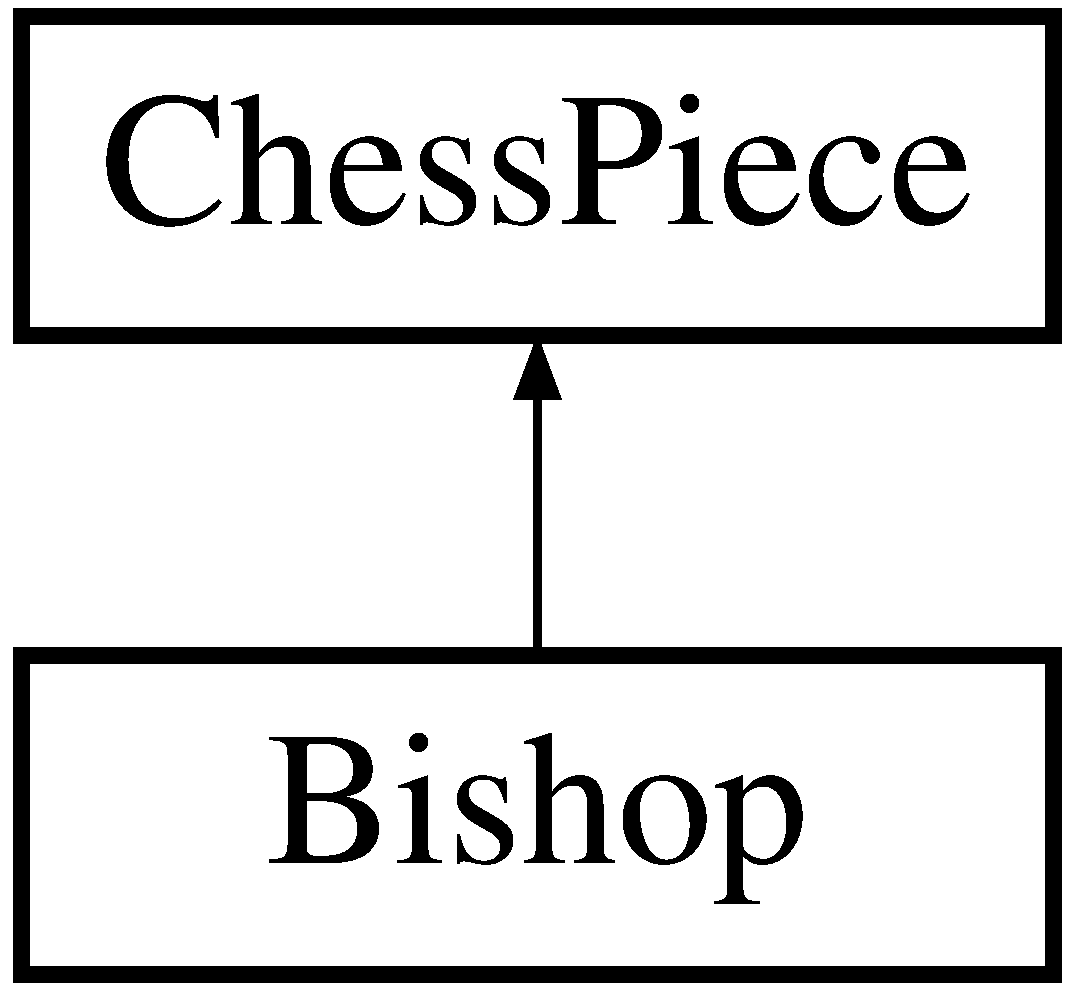
\includegraphics[height=2.000000cm]{class_bishop}
\end{center}
\end{figure}
\subsection*{Public Member Functions}
\begin{DoxyCompactItemize}
\item 
\mbox{\Hypertarget{class_bishop_a06f0625981bd2448de46b99edb4afb00}\label{class_bishop_a06f0625981bd2448de46b99edb4afb00}} 
{\bfseries Bishop} (\mbox{\hyperlink{class_board}{Board}} $\ast$board, \mbox{\hyperlink{class_square}{Square}} $\ast$location, Piece\+Color color)
\item 
\mbox{\Hypertarget{class_bishop_a2239bc73616d1545289e55f3ee6b686d}\label{class_bishop_a2239bc73616d1545289e55f3ee6b686d}} 
std\+::vector$<$ \mbox{\hyperlink{class_square}{Square}} $\ast$ $>$ {\bfseries get\+Available\+Squares} (bool consider\+Check) override
\end{DoxyCompactItemize}
\subsection*{Additional Inherited Members}


The documentation for this class was generated from the following files\+:\begin{DoxyCompactItemize}
\item 
chesspieces/Bishop.\+h\item 
chesspieces/Bishop.\+cpp\end{DoxyCompactItemize}

\hypertarget{class_board}{}\section{Board Class Reference}
\label{class_board}\index{Board@{Board}}
\subsection*{Public Member Functions}
\begin{DoxyCompactItemize}
\item 
\mbox{\Hypertarget{class_board_a585c430e82e9e53020dbb503acd7b5b9}\label{class_board_a585c430e82e9e53020dbb503acd7b5b9}} 
{\bfseries Board} (Render\+Window \&window)
\item 
\mbox{\Hypertarget{class_board_a167d2711ebed12b7f66563893a86e68f}\label{class_board_a167d2711ebed12b7f66563893a86e68f}} 
{\bfseries Board} (\mbox{\hyperlink{class_board}{Board}} const \&)=default
\item 
\mbox{\Hypertarget{class_board_a1845216283a171939dcb477dce3a17b8}\label{class_board_a1845216283a171939dcb477dce3a17b8}} 
void {\bfseries draw\+Board} ()
\item 
\mbox{\Hypertarget{class_board_a4ae06b15573b9e33e3c0821aaa297443}\label{class_board_a4ae06b15573b9e33e3c0821aaa297443}} 
void {\bfseries start\+Game} (\mbox{\hyperlink{class_player}{Player}} $\ast$bottom\+Player, \mbox{\hyperlink{class_player}{Player}} $\ast$top\+Player, \mbox{\hyperlink{class_player}{Player}} $\ast$current\+Player)
\item 
\mbox{\Hypertarget{class_board_ad879f0bb4294839df986a4c228608b54}\label{class_board_ad879f0bb4294839df986a4c228608b54}} 
void {\bfseries select\+Square\+From\+Coordinates} (Vector2i coordinates)
\item 
\mbox{\Hypertarget{class_board_a2d11c7b0de1e2b9a8137bf6c3bdd2528}\label{class_board_a2d11c7b0de1e2b9a8137bf6c3bdd2528}} 
void {\bfseries focus\+Squares} ()
\item 
\mbox{\Hypertarget{class_board_ae50158d0fdb0b1facb38809366cdc07b}\label{class_board_ae50158d0fdb0b1facb38809366cdc07b}} 
void {\bfseries do\+Move} (\mbox{\hyperlink{class_move}{Move}} $\ast$next\+Move)
\item 
\mbox{\Hypertarget{class_board_ae4186ea27fa755a8b4f3340a187dbb84}\label{class_board_ae4186ea27fa755a8b4f3340a187dbb84}} 
void {\bfseries set\+Current\+Player} (\mbox{\hyperlink{class_player}{Player}} $\ast$current\+Player)
\item 
\mbox{\Hypertarget{class_board_ad64ef35c0f386828624f96502180f28b}\label{class_board_ad64ef35c0f386828624f96502180f28b}} 
void {\bfseries undo\+Move} ()
\item 
\mbox{\Hypertarget{class_board_a4c93238f3c9d66b420da8e8ab4827dec}\label{class_board_a4c93238f3c9d66b420da8e8ab4827dec}} 
void {\bfseries check\+Game\+Status} ()
\item 
\mbox{\Hypertarget{class_board_ac9209dfee06d62e24e84f72ae97b2fe2}\label{class_board_ac9209dfee06d62e24e84f72ae97b2fe2}} 
std\+::vector$<$ \mbox{\hyperlink{class_chess_piece}{Chess\+Piece}} $\ast$ $>$ {\bfseries get\+Pieces\+By\+Color} (Piece\+Color color)
\item 
\mbox{\Hypertarget{class_board_a858ccf256bfd728f0dca7397c4a5c5f5}\label{class_board_a858ccf256bfd728f0dca7397c4a5c5f5}} 
bool {\bfseries is\+In\+Check} (Piece\+Color color)
\item 
\mbox{\Hypertarget{class_board_ad30b52d82ee21488c1f43f3ee13978c1}\label{class_board_ad30b52d82ee21488c1f43f3ee13978c1}} 
bool {\bfseries check\+Mate} ()
\end{DoxyCompactItemize}
\subsection*{Public Attributes}
\begin{DoxyCompactItemize}
\item 
\mbox{\Hypertarget{class_board_a99ddd88853d01027c7e903b97391ce02}\label{class_board_a99ddd88853d01027c7e903b97391ce02}} 
\mbox{\hyperlink{class_square}{Square}} $\ast$ {\bfseries squares} \mbox{[}8\mbox{]}\mbox{[}8\mbox{]}
\item 
\mbox{\Hypertarget{class_board_a0b713008789cb6fb39e1d9b848997aa9}\label{class_board_a0b713008789cb6fb39e1d9b848997aa9}} 
std\+::vector$<$ \mbox{\hyperlink{class_move}{Move}} $\ast$ $>$ {\bfseries all\+Moves}
\item 
\mbox{\Hypertarget{class_board_a4db7733c8dab61d734c5f0e29a46e72f}\label{class_board_a4db7733c8dab61d734c5f0e29a46e72f}} 
\mbox{\hyperlink{class_square}{Square}} $\ast$ {\bfseries selected\+Square}
\item 
\mbox{\Hypertarget{class_board_ad5e605d5c3319a4c0758fb27ec94d81f}\label{class_board_ad5e605d5c3319a4c0758fb27ec94d81f}} 
\mbox{\hyperlink{class_player}{Player}} $\ast$ {\bfseries bottom\+Player}
\item 
\mbox{\Hypertarget{class_board_ad64f2c022585c3f83f5963983f745446}\label{class_board_ad64f2c022585c3f83f5963983f745446}} 
\mbox{\hyperlink{class_player}{Player}} $\ast$ {\bfseries top\+Player}
\item 
\mbox{\Hypertarget{class_board_a07865ff5631b2a9a236234acc57e9b5d}\label{class_board_a07865ff5631b2a9a236234acc57e9b5d}} 
\mbox{\hyperlink{class_player}{Player}} $\ast$ {\bfseries current\+Player}
\end{DoxyCompactItemize}


The documentation for this class was generated from the following files\+:\begin{DoxyCompactItemize}
\item 
Board.\+h\item 
Board.\+cpp\end{DoxyCompactItemize}

\hypertarget{class_chess_piece}{}\section{Chess\+Piece Class Reference}
\label{class_chess_piece}\index{Chess\+Piece@{Chess\+Piece}}
Inheritance diagram for Chess\+Piece\+:\begin{figure}[H]
\begin{center}
\leavevmode
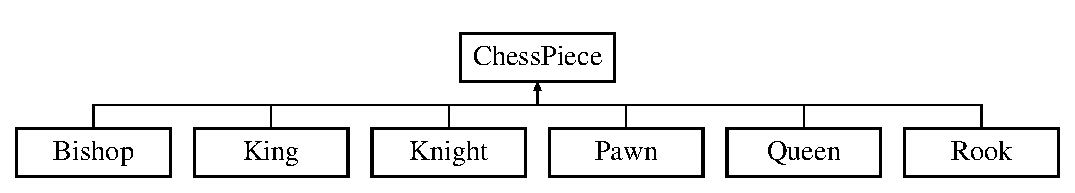
\includegraphics[height=2.000000cm]{class_chess_piece}
\end{center}
\end{figure}
\subsection*{Public Member Functions}
\begin{DoxyCompactItemize}
\item 
\mbox{\Hypertarget{class_chess_piece_a4a74c820a7e6999ba71184bb4b276782}\label{class_chess_piece_a4a74c820a7e6999ba71184bb4b276782}} 
{\bfseries Chess\+Piece} (\mbox{\hyperlink{class_board}{Board}} $\ast$board, \mbox{\hyperlink{class_square}{Square}} $\ast$location, Piece\+Color color)
\item 
\mbox{\Hypertarget{class_chess_piece_aca89f884439b41fb8e5810d5c2a798fc}\label{class_chess_piece_aca89f884439b41fb8e5810d5c2a798fc}} 
void {\bfseries draw\+Chess\+Piece} (sf\+::\+Render\+Window \&window)
\item 
\mbox{\Hypertarget{class_chess_piece_a864599823fa1735a1ddda632beb97bbb}\label{class_chess_piece_a864599823fa1735a1ddda632beb97bbb}} 
virtual std\+::vector$<$ \mbox{\hyperlink{class_square}{Square}} $\ast$ $>$ {\bfseries get\+Available\+Squares} (bool consider\+Check)=0
\item 
\mbox{\Hypertarget{class_chess_piece_ad071550868f5c48aec1a5e4a3cb5ed6f}\label{class_chess_piece_ad071550868f5c48aec1a5e4a3cb5ed6f}} 
virtual std\+::vector$<$ \mbox{\hyperlink{class_move}{Move}} $\ast$ $>$ {\bfseries get\+Available\+Moves} (bool consider\+Check)
\item 
\mbox{\Hypertarget{class_chess_piece_a712fb4fa01285d525c256e9da2787031}\label{class_chess_piece_a712fb4fa01285d525c256e9da2787031}} 
virtual int {\bfseries get\+Location\+Score} (int x, int y)
\end{DoxyCompactItemize}
\subsection*{Public Attributes}
\begin{DoxyCompactItemize}
\item 
\mbox{\Hypertarget{class_chess_piece_a3e2de896951ca2959cd4106150779d79}\label{class_chess_piece_a3e2de896951ca2959cd4106150779d79}} 
Piece\+Type {\bfseries type}
\item 
\mbox{\Hypertarget{class_chess_piece_ae193a49a5fd0430bc047e50801f2077d}\label{class_chess_piece_ae193a49a5fd0430bc047e50801f2077d}} 
\mbox{\hyperlink{class_board}{Board}} $\ast$ {\bfseries board}
\item 
\mbox{\Hypertarget{class_chess_piece_af82d56d5d5da9afa1e2c2890dda6b29e}\label{class_chess_piece_af82d56d5d5da9afa1e2c2890dda6b29e}} 
\mbox{\hyperlink{class_square}{Square}} $\ast$ {\bfseries location}
\item 
\mbox{\Hypertarget{class_chess_piece_a19c89a7de4c1936528c11c393480aa1a}\label{class_chess_piece_a19c89a7de4c1936528c11c393480aa1a}} 
Piece\+Color {\bfseries color}
\item 
\mbox{\Hypertarget{class_chess_piece_a13150134984c3912b61bf19e0b0b0ca3}\label{class_chess_piece_a13150134984c3912b61bf19e0b0b0ca3}} 
int {\bfseries amount\+Of\+Steps} = 0
\item 
\mbox{\Hypertarget{class_chess_piece_a14617579ee81691cb019ce59d2be1289}\label{class_chess_piece_a14617579ee81691cb019ce59d2be1289}} 
bool {\bfseries is\+Checked} = false
\item 
\mbox{\Hypertarget{class_chess_piece_ae4c2a1cf92fa38967b42e17068738f3a}\label{class_chess_piece_ae4c2a1cf92fa38967b42e17068738f3a}} 
bool {\bfseries is\+Captured} = false
\item 
\mbox{\Hypertarget{class_chess_piece_afe9c6ae949d443f106617d2e588fe532}\label{class_chess_piece_afe9c6ae949d443f106617d2e588fe532}} 
int {\bfseries piece\+Score}
\item 
\mbox{\Hypertarget{class_chess_piece_a55b7732f3c4f7c3636092b05e685d2f6}\label{class_chess_piece_a55b7732f3c4f7c3636092b05e685d2f6}} 
std\+::array$<$ std\+::array$<$ int, 8 $>$, 8 $>$ {\bfseries location\+Scores}
\end{DoxyCompactItemize}
\subsection*{Protected Member Functions}
\begin{DoxyCompactItemize}
\item 
\mbox{\Hypertarget{class_chess_piece_a3918de640f232f48572dc16ccc7b46ad}\label{class_chess_piece_a3918de640f232f48572dc16ccc7b46ad}} 
std\+::vector$<$ \mbox{\hyperlink{class_square}{Square}} $\ast$ $>$ {\bfseries remove\+Moves\+Leading\+To\+Self\+Check} (std\+::vector$<$ \mbox{\hyperlink{class_square}{Square}} $\ast$$>$ moves)
\item 
\mbox{\Hypertarget{class_chess_piece_a474443b35ab57036945c9d72ffba5676}\label{class_chess_piece_a474443b35ab57036945c9d72ffba5676}} 
std\+::vector$<$ \mbox{\hyperlink{class_square}{Square}} $\ast$ $>$ {\bfseries calculate\+Moves\+For\+Directions} (\mbox{\hyperlink{class_square}{Square}} $\ast$location, Vector2i directions\mbox{[}$\,$\mbox{]}, \mbox{\hyperlink{class_board}{Board}} $\ast$board, Piece\+Color color, short amount\+Of\+Directions, short max\+Amount\+Of\+Steps, bool consider\+Check)
\item 
\mbox{\Hypertarget{class_chess_piece_a516757b5d6cc1a37a44d4cc859cdb2b8}\label{class_chess_piece_a516757b5d6cc1a37a44d4cc859cdb2b8}} 
void {\bfseries generate\+Image} (Piece\+Type type)
\end{DoxyCompactItemize}


The documentation for this class was generated from the following files\+:\begin{DoxyCompactItemize}
\item 
Chess\+Piece.\+h\item 
Chess\+Piece.\+cpp\end{DoxyCompactItemize}

\hypertarget{class_human_player}{}\section{Human\+Player Class Reference}
\label{class_human_player}\index{Human\+Player@{Human\+Player}}
Inheritance diagram for Human\+Player\+:\begin{figure}[H]
\begin{center}
\leavevmode
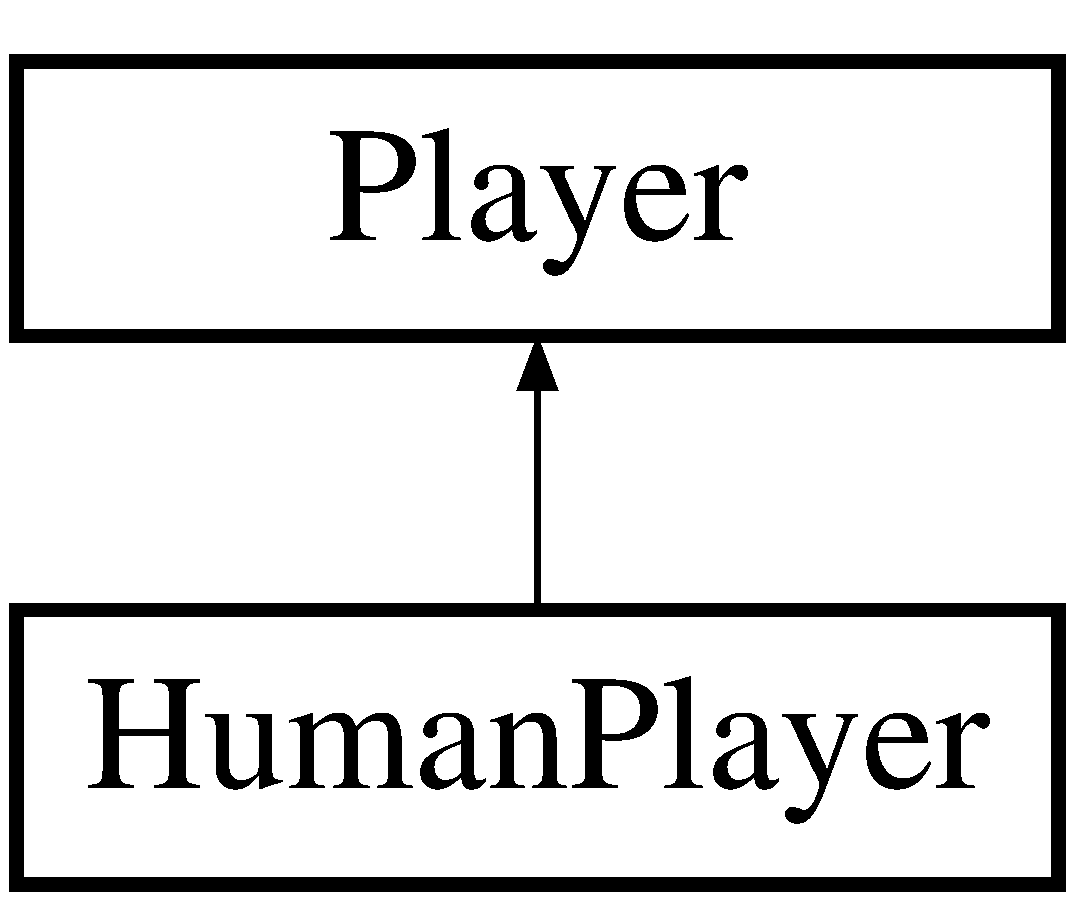
\includegraphics[height=2.000000cm]{class_human_player}
\end{center}
\end{figure}
\subsection*{Public Member Functions}
\begin{DoxyCompactItemize}
\item 
\mbox{\Hypertarget{class_human_player_a9126eadf60fc35c400d656610e288eda}\label{class_human_player_a9126eadf60fc35c400d656610e288eda}} 
{\bfseries Human\+Player} (sf\+::\+Render\+Window \&window)
\item 
\mbox{\Hypertarget{class_human_player_a36d914c4805583851031fc3d537d0cd5}\label{class_human_player_a36d914c4805583851031fc3d537d0cd5}} 
{\bfseries Human\+Player} (Piece\+Color color, sf\+::\+Render\+Window \&window)
\item 
\mbox{\Hypertarget{class_human_player_abd281d6f332ccfeaf4e8f5b330a496f8}\label{class_human_player_abd281d6f332ccfeaf4e8f5b330a496f8}} 
\mbox{\hyperlink{class_move}{Move}} $\ast$ {\bfseries get\+Next\+Move} (\mbox{\hyperlink{class_board}{Board}} $\ast$board)
\end{DoxyCompactItemize}
\subsection*{Additional Inherited Members}


The documentation for this class was generated from the following files\+:\begin{DoxyCompactItemize}
\item 
players/Human\+Player.\+h\item 
players/Human\+Player.\+cpp\end{DoxyCompactItemize}

\hypertarget{class_interface}{}\section{Interface Class Reference}
\label{class_interface}\index{Interface@{Interface}}
\subsection*{Public Member Functions}
\begin{DoxyCompactItemize}
\item 
\mbox{\Hypertarget{class_interface_afe5bec89bb6b1b22ac826169eff10b31}\label{class_interface_afe5bec89bb6b1b22ac826169eff10b31}} 
{\bfseries Interface} (Render\+Window \&window, \mbox{\hyperlink{class_board}{Board}} \&board)
\item 
\mbox{\Hypertarget{class_interface_a89d04c54dcf70d05c942b0e8ddce51f1}\label{class_interface_a89d04c54dcf70d05c942b0e8ddce51f1}} 
void {\bfseries show\+Current\+Player\+Text} (\mbox{\hyperlink{class_player}{Player}} $\ast$current\+Player)
\item 
\mbox{\Hypertarget{class_interface_a261b7350edcb97bf5deb61cb548a39e6}\label{class_interface_a261b7350edcb97bf5deb61cb548a39e6}} 
void {\bfseries show\+Selected\+Square\+Name} ()
\item 
\mbox{\Hypertarget{class_interface_a769d9f7977a2917fe7752b355e1946fa}\label{class_interface_a769d9f7977a2917fe7752b355e1946fa}} 
void {\bfseries show\+Player\+Types} ()
\item 
\mbox{\Hypertarget{class_interface_af231aba8f4addf49b7e581bf99bb80cb}\label{class_interface_af231aba8f4addf49b7e581bf99bb80cb}} 
void {\bfseries show\+Coordinates} ()
\item 
\mbox{\Hypertarget{class_interface_a8991fc674d8298e9b9e83977a2c3386a}\label{class_interface_a8991fc674d8298e9b9e83977a2c3386a}} 
void {\bfseries show\+Board\+Background} ()
\end{DoxyCompactItemize}


The documentation for this class was generated from the following files\+:\begin{DoxyCompactItemize}
\item 
Interface.\+h\item 
Interface.\+cpp\end{DoxyCompactItemize}

\hypertarget{class_king}{}\section{King Class Reference}
\label{class_king}\index{King@{King}}
Inheritance diagram for King\+:\begin{figure}[H]
\begin{center}
\leavevmode
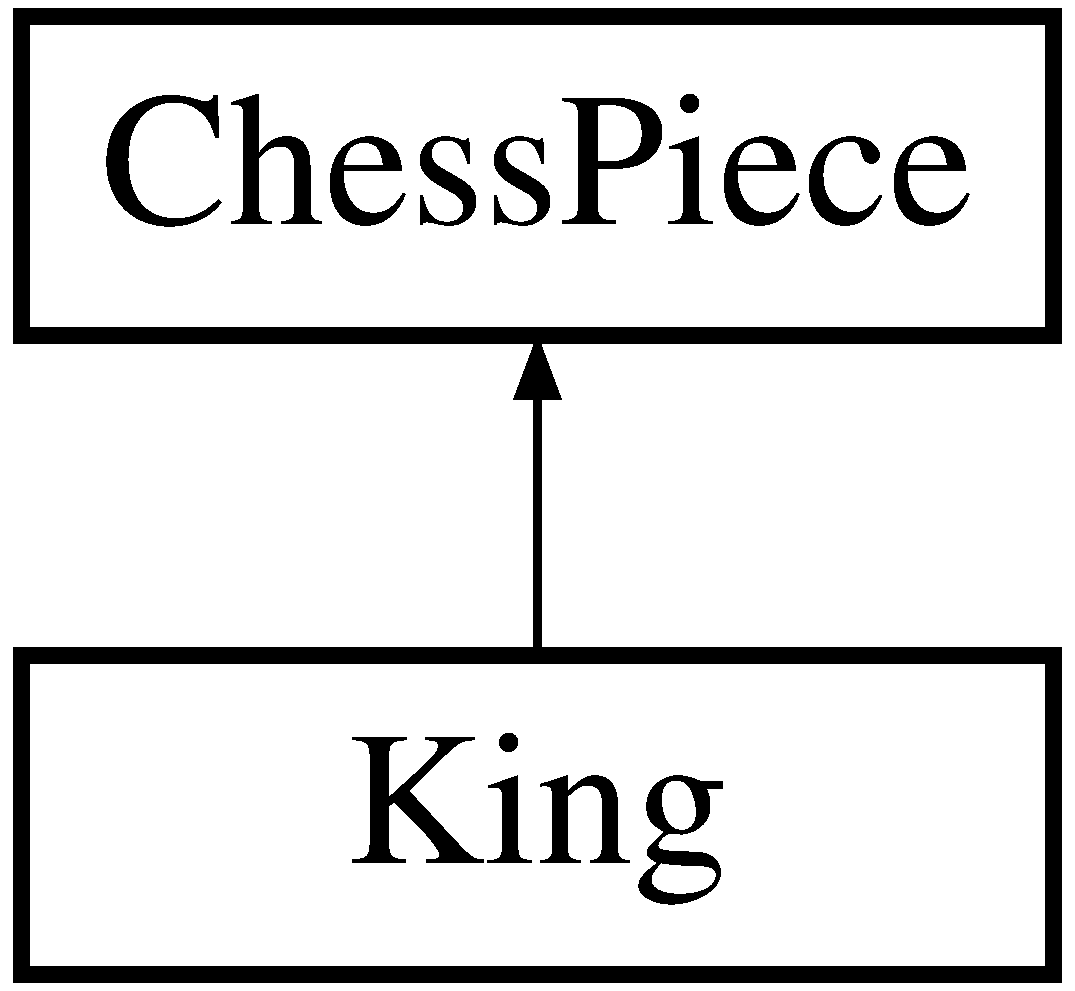
\includegraphics[height=2.000000cm]{class_king}
\end{center}
\end{figure}
\subsection*{Public Member Functions}
\begin{DoxyCompactItemize}
\item 
\mbox{\Hypertarget{class_king_aadb14b6b3940ffa4b824a7d48cdb5432}\label{class_king_aadb14b6b3940ffa4b824a7d48cdb5432}} 
{\bfseries King} (\mbox{\hyperlink{class_board}{Board}} $\ast$board, \mbox{\hyperlink{class_square}{Square}} $\ast$location, Piece\+Color color)
\item 
\mbox{\Hypertarget{class_king_a84fa2e4cc019a050ec0b973b51915710}\label{class_king_a84fa2e4cc019a050ec0b973b51915710}} 
std\+::vector$<$ \mbox{\hyperlink{class_square}{Square}} $\ast$ $>$ {\bfseries get\+Available\+Squares} (bool consider\+Check) override
\item 
\mbox{\Hypertarget{class_king_a9a4b9b423ae1bf7b9d199f411addaebc}\label{class_king_a9a4b9b423ae1bf7b9d199f411addaebc}} 
std\+::vector$<$ \mbox{\hyperlink{class_move}{Move}} $\ast$ $>$ {\bfseries add\+Castling\+Moves} (std\+::vector$<$ \mbox{\hyperlink{class_move}{Move}} $\ast$$>$ moves, bool consider\+Check)
\item 
\mbox{\Hypertarget{class_king_a7cb7eec2bcc39f107c9e91a382881bdc}\label{class_king_a7cb7eec2bcc39f107c9e91a382881bdc}} 
std\+::vector$<$ \mbox{\hyperlink{class_move}{Move}} $\ast$ $>$ {\bfseries get\+Available\+Moves} (bool consider\+Check) override
\end{DoxyCompactItemize}
\subsection*{Additional Inherited Members}


The documentation for this class was generated from the following files\+:\begin{DoxyCompactItemize}
\item 
chesspieces/King.\+h\item 
chesspieces/King.\+cpp\end{DoxyCompactItemize}

\hypertarget{class_knight}{}\section{Knight Class Reference}
\label{class_knight}\index{Knight@{Knight}}
Inheritance diagram for Knight\+:\begin{figure}[H]
\begin{center}
\leavevmode
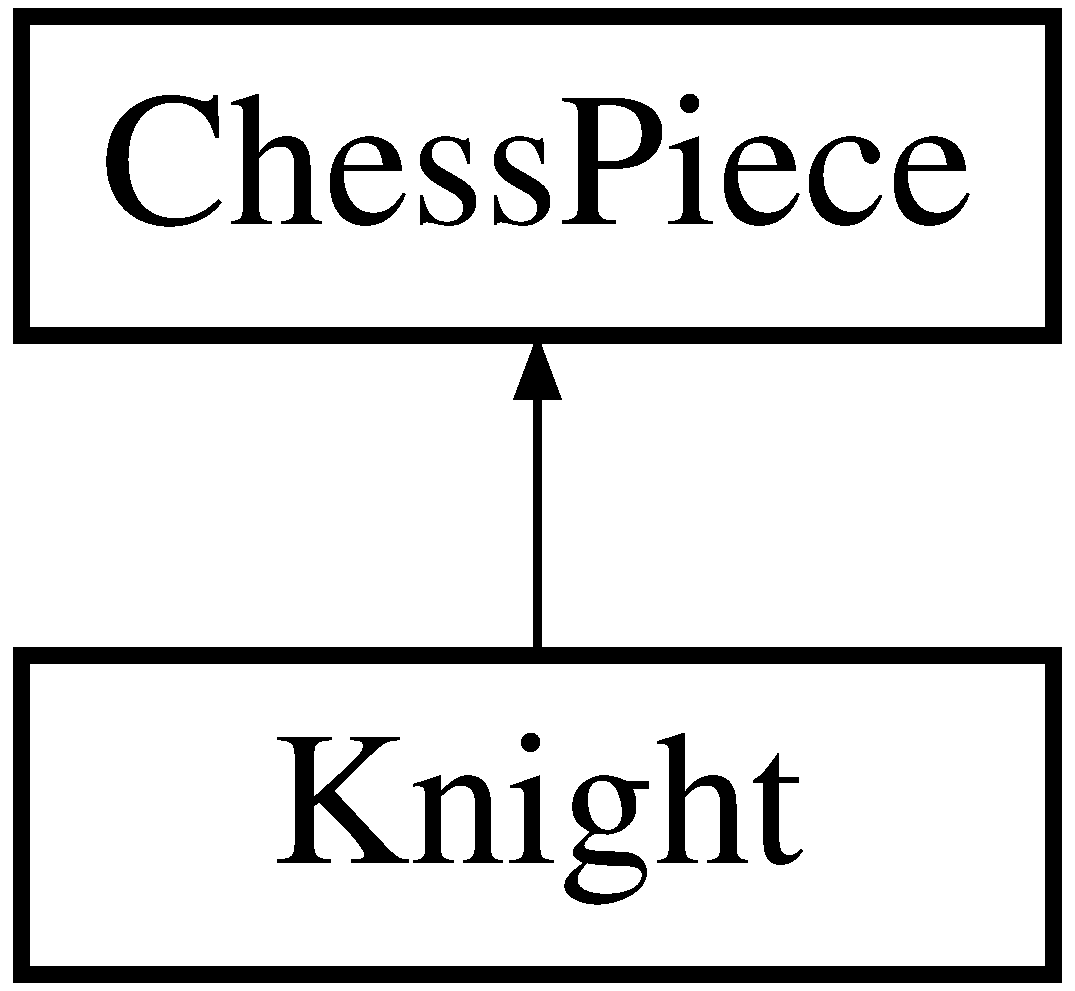
\includegraphics[height=2.000000cm]{class_knight}
\end{center}
\end{figure}
\subsection*{Public Member Functions}
\begin{DoxyCompactItemize}
\item 
\mbox{\Hypertarget{class_knight_a05aa3fb92b9791437b3ab86b8f2865f4}\label{class_knight_a05aa3fb92b9791437b3ab86b8f2865f4}} 
{\bfseries Knight} (\mbox{\hyperlink{class_board}{Board}} $\ast$board, \mbox{\hyperlink{class_square}{Square}} $\ast$location, Piece\+Color color)
\item 
\mbox{\Hypertarget{class_knight_ae64ee94abb50171423efc7608a2337ca}\label{class_knight_ae64ee94abb50171423efc7608a2337ca}} 
std\+::vector$<$ \mbox{\hyperlink{class_square}{Square}} $\ast$ $>$ {\bfseries get\+Available\+Squares} (bool consider\+Check)
\end{DoxyCompactItemize}
\subsection*{Additional Inherited Members}


The documentation for this class was generated from the following files\+:\begin{DoxyCompactItemize}
\item 
chesspieces/Knight.\+h\item 
chesspieces/Knight.\+cpp\end{DoxyCompactItemize}

\hypertarget{class_min_max_player}{}\section{Min\+Max\+Player Class Reference}
\label{class_min_max_player}\index{Min\+Max\+Player@{Min\+Max\+Player}}
Inheritance diagram for Min\+Max\+Player\+:\begin{figure}[H]
\begin{center}
\leavevmode
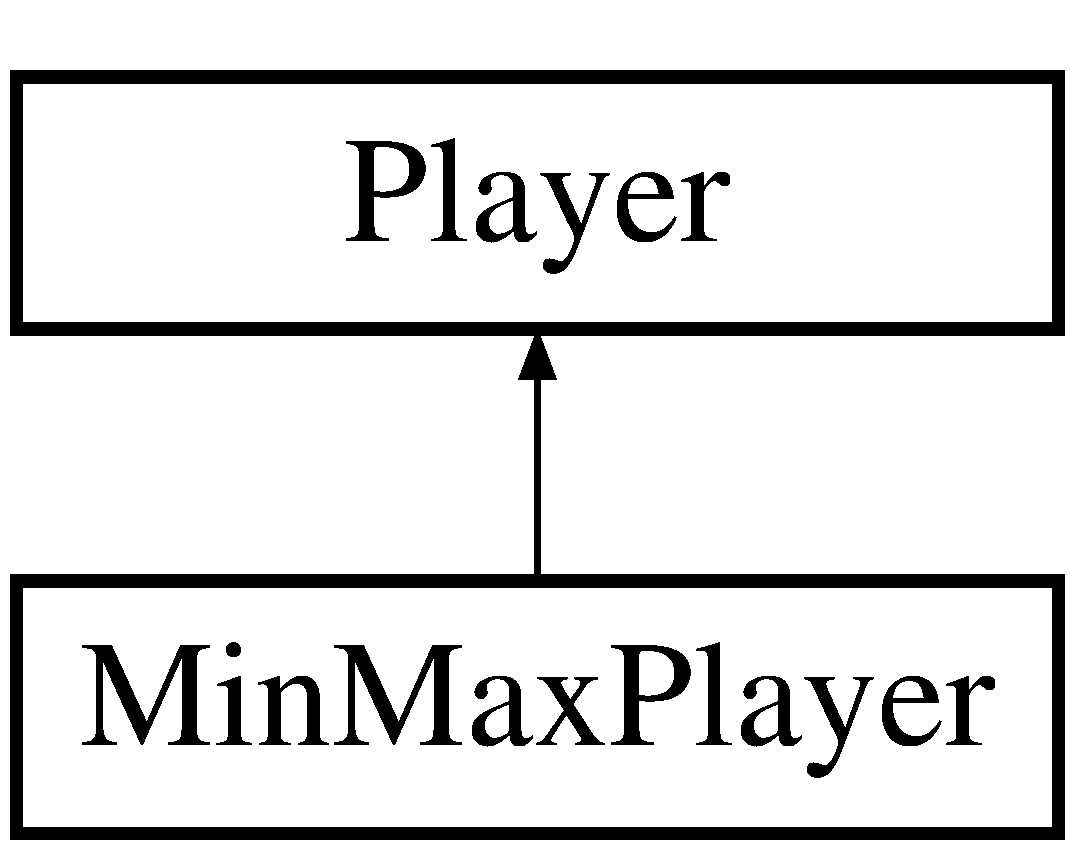
\includegraphics[height=2.000000cm]{class_min_max_player}
\end{center}
\end{figure}
\subsection*{Public Member Functions}
\begin{DoxyCompactItemize}
\item 
\mbox{\Hypertarget{class_min_max_player_a145255a37fa1c12d9cd0db6c132732b6}\label{class_min_max_player_a145255a37fa1c12d9cd0db6c132732b6}} 
{\bfseries Min\+Max\+Player} (Piece\+Color color)
\item 
\mbox{\Hypertarget{class_min_max_player_a1330801ee17c3acce9d3245d27bd41a6}\label{class_min_max_player_a1330801ee17c3acce9d3245d27bd41a6}} 
\mbox{\hyperlink{class_move}{Move}} $\ast$ {\bfseries get\+Next\+Move} (\mbox{\hyperlink{class_board}{Board}} $\ast$board)
\item 
\mbox{\Hypertarget{class_min_max_player_aedd032551771faa29a729d0733e9cab4}\label{class_min_max_player_aedd032551771faa29a729d0733e9cab4}} 
long {\bfseries get\+Move\+Score} (\mbox{\hyperlink{class_board}{Board}} $\ast$, \mbox{\hyperlink{class_move}{Move}} $\ast$, Piece\+Color, int, long, long)
\item 
\mbox{\Hypertarget{class_min_max_player_a75472f13216313417a63c55aa493522b}\label{class_min_max_player_a75472f13216313417a63c55aa493522b}} 
\mbox{\hyperlink{class_move}{Move}} $\ast$ {\bfseries determine\+Move} (\mbox{\hyperlink{class_board}{Board}} $\ast$, Piece\+Color)
\end{DoxyCompactItemize}
\subsection*{Additional Inherited Members}


The documentation for this class was generated from the following files\+:\begin{DoxyCompactItemize}
\item 
players/Min\+Max\+Player.\+h\item 
players/Min\+Max\+Player.\+cpp\end{DoxyCompactItemize}

\hypertarget{class_move}{}\section{Move Class Reference}
\label{class_move}\index{Move@{Move}}
\subsection*{Public Member Functions}
\begin{DoxyCompactItemize}
\item 
\mbox{\Hypertarget{class_move_a38c4990ac28b0cdfae9050409ab7415a}\label{class_move_a38c4990ac28b0cdfae9050409ab7415a}} 
{\bfseries Move} (\mbox{\hyperlink{class_board}{Board}} $\ast$, \mbox{\hyperlink{class_square}{Square}} $\ast$, \mbox{\hyperlink{class_square}{Square}} $\ast$)
\item 
\mbox{\Hypertarget{class_move_acefd7884211b1f7a7d2b8ba4ddcf1ba9}\label{class_move_acefd7884211b1f7a7d2b8ba4ddcf1ba9}} 
{\bfseries Move} (\mbox{\hyperlink{class_board}{Board}} $\ast$, \mbox{\hyperlink{class_square}{Square}} $\ast$, \mbox{\hyperlink{class_square}{Square}} $\ast$, bool)
\item 
\mbox{\Hypertarget{class_move_a904562de252b165c26c1f139d259c8eb}\label{class_move_a904562de252b165c26c1f139d259c8eb}} 
{\bfseries Move} (\mbox{\hyperlink{class_board}{Board}} $\ast$, \mbox{\hyperlink{class_square}{Square}} $\ast$, \mbox{\hyperlink{class_square}{Square}} $\ast$, bool, Castling\+Side, \mbox{\hyperlink{class_chess_piece}{Chess\+Piece}} $\ast$, \mbox{\hyperlink{class_square}{Square}} $\ast$, \mbox{\hyperlink{class_square}{Square}} $\ast$)
\item 
\mbox{\Hypertarget{class_move_a9d91dd03207b55a7016a5f8de36f698a}\label{class_move_a9d91dd03207b55a7016a5f8de36f698a}} 
void {\bfseries generate\+Name} ()
\end{DoxyCompactItemize}
\subsection*{Public Attributes}
\begin{DoxyCompactItemize}
\item 
\mbox{\Hypertarget{class_move_adcbbe513c87c0dcc19f05619973a3b1d}\label{class_move_adcbbe513c87c0dcc19f05619973a3b1d}} 
\mbox{\hyperlink{class_square}{Square}} $\ast$ {\bfseries start\+Of\+Move}
\item 
\mbox{\Hypertarget{class_move_a4e8eb6c451062b79d880ce3d346e20af}\label{class_move_a4e8eb6c451062b79d880ce3d346e20af}} 
\mbox{\hyperlink{class_square}{Square}} $\ast$ {\bfseries end\+Of\+Move}
\item 
\mbox{\Hypertarget{class_move_a2f179bb489b6f1a14830e1e81b5eccfd}\label{class_move_a2f179bb489b6f1a14830e1e81b5eccfd}} 
\mbox{\hyperlink{class_chess_piece}{Chess\+Piece}} $\ast$ {\bfseries initial\+Piece}
\item 
\mbox{\Hypertarget{class_move_adcc5fa48f045b094b32cd8f902d57acd}\label{class_move_adcc5fa48f045b094b32cd8f902d57acd}} 
\mbox{\hyperlink{class_chess_piece}{Chess\+Piece}} $\ast$ {\bfseries taken\+Piece}
\item 
\mbox{\Hypertarget{class_move_a1fbc388e091cd5639b755ebca2a8f90b}\label{class_move_a1fbc388e091cd5639b755ebca2a8f90b}} 
\mbox{\hyperlink{class_player}{Player}} $\ast$ {\bfseries player}
\item 
\mbox{\Hypertarget{class_move_a8861c7af9b982677666292f88c06029d}\label{class_move_a8861c7af9b982677666292f88c06029d}} 
bool {\bfseries is\+Simulated} = false
\item 
\mbox{\Hypertarget{class_move_aeb167ac5b5026207799035ea00467a20}\label{class_move_aeb167ac5b5026207799035ea00467a20}} 
std\+::string {\bfseries name}
\item 
\mbox{\Hypertarget{class_move_a264e68c2f070d39c895889b2edfc66b0}\label{class_move_a264e68c2f070d39c895889b2edfc66b0}} 
Castling\+Side {\bfseries castling\+Side}
\item 
\mbox{\Hypertarget{class_move_a6a0dc44a92343f6f0f951df9d2c5add3}\label{class_move_a6a0dc44a92343f6f0f951df9d2c5add3}} 
\mbox{\hyperlink{class_chess_piece}{Chess\+Piece}} $\ast$ {\bfseries castling\+Rook} = nullptr
\item 
\mbox{\Hypertarget{class_move_aa904a23353053bc9a8c963828a89e032}\label{class_move_aa904a23353053bc9a8c963828a89e032}} 
\mbox{\hyperlink{class_square}{Square}} $\ast$ {\bfseries rook\+Target\+Square} = nullptr
\item 
\mbox{\Hypertarget{class_move_a0be40463b39204457c4c2a331403ad49}\label{class_move_a0be40463b39204457c4c2a331403ad49}} 
\mbox{\hyperlink{class_square}{Square}} $\ast$ {\bfseries inital\+Rook\+Square} = nullptr
\item 
\mbox{\Hypertarget{class_move_a07f0eb12d13ed4f65c0dcc65946f583c}\label{class_move_a07f0eb12d13ed4f65c0dcc65946f583c}} 
bool {\bfseries is\+Promoting} = false
\item 
\mbox{\Hypertarget{class_move_ae947bead41a531a56957916b007cdfb4}\label{class_move_ae947bead41a531a56957916b007cdfb4}} 
\mbox{\hyperlink{class_chess_piece}{Chess\+Piece}} $\ast$ {\bfseries promoted\+Piece} = nullptr
\item 
\mbox{\Hypertarget{class_move_a8373efdfa68c28e953d337b95b946c08}\label{class_move_a8373efdfa68c28e953d337b95b946c08}} 
\mbox{\hyperlink{class_chess_piece}{Chess\+Piece}} $\ast$ {\bfseries en\+Passant\+Taken\+Piece} = nullptr
\end{DoxyCompactItemize}


The documentation for this class was generated from the following files\+:\begin{DoxyCompactItemize}
\item 
Move.\+h\item 
Move.\+cpp\end{DoxyCompactItemize}

\hypertarget{class_pawn}{}\section{Pawn Class Reference}
\label{class_pawn}\index{Pawn@{Pawn}}
Inheritance diagram for Pawn\+:\begin{figure}[H]
\begin{center}
\leavevmode
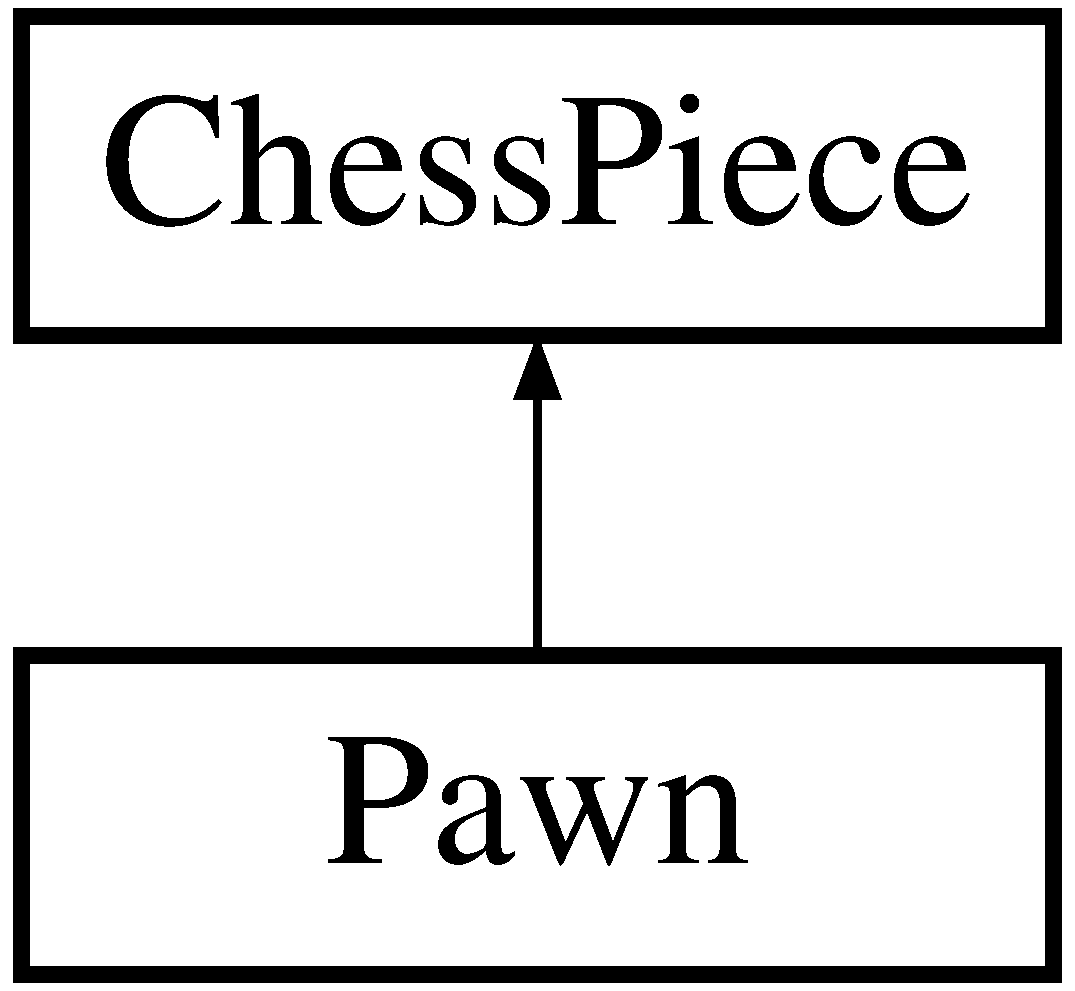
\includegraphics[height=2.000000cm]{class_pawn}
\end{center}
\end{figure}
\subsection*{Public Member Functions}
\begin{DoxyCompactItemize}
\item 
\mbox{\Hypertarget{class_pawn_a916ab319cd46b42afa364dd1f05895bf}\label{class_pawn_a916ab319cd46b42afa364dd1f05895bf}} 
{\bfseries Pawn} (\mbox{\hyperlink{class_board}{Board}} $\ast$, \mbox{\hyperlink{class_square}{Square}} $\ast$, Piece\+Color)
\item 
\mbox{\Hypertarget{class_pawn_a11d2b85c7aa36107a2025aa3bf0a9fbb}\label{class_pawn_a11d2b85c7aa36107a2025aa3bf0a9fbb}} 
vector$<$ \mbox{\hyperlink{class_square}{Square}} $\ast$ $>$ {\bfseries get\+Available\+Squares} (bool)
\item 
\mbox{\Hypertarget{class_pawn_a16066f4c1d424d7843af4cb4ffc01594}\label{class_pawn_a16066f4c1d424d7843af4cb4ffc01594}} 
vector$<$ \mbox{\hyperlink{class_move}{Move}} $\ast$ $>$ {\bfseries get\+Available\+Moves} (bool) override
\item 
\mbox{\Hypertarget{class_pawn_a62f439391ed8f3b37d191248f80ae022}\label{class_pawn_a62f439391ed8f3b37d191248f80ae022}} 
vector$<$ \mbox{\hyperlink{class_move}{Move}} $\ast$ $>$ {\bfseries add\+En\+Passant\+Moves} (vector$<$ \mbox{\hyperlink{class_move}{Move}} $\ast$$>$)
\end{DoxyCompactItemize}
\subsection*{Additional Inherited Members}


The documentation for this class was generated from the following files\+:\begin{DoxyCompactItemize}
\item 
chesspieces/Pawn.\+h\item 
chesspieces/Pawn.\+cpp\end{DoxyCompactItemize}

\hypertarget{class_player}{}\section{Player Class Reference}
\label{class_player}\index{Player@{Player}}
Inheritance diagram for Player\+:\begin{figure}[H]
\begin{center}
\leavevmode
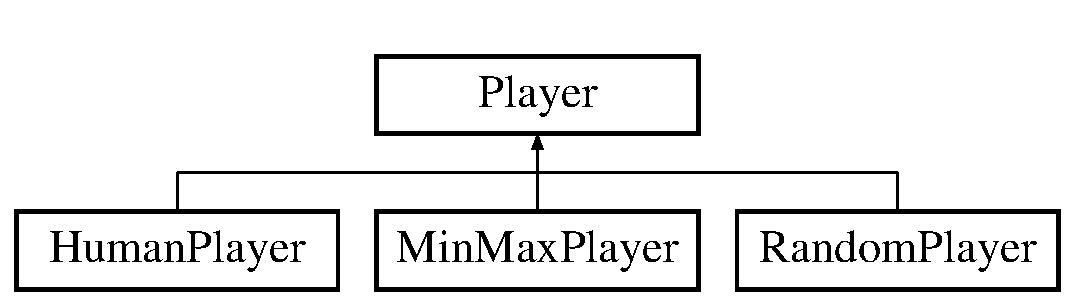
\includegraphics[height=2.000000cm]{class_player}
\end{center}
\end{figure}
\subsection*{Public Member Functions}
\begin{DoxyCompactItemize}
\item 
\mbox{\Hypertarget{class_player_ab89c7040e9d3c84a557992039ee10418}\label{class_player_ab89c7040e9d3c84a557992039ee10418}} 
{\bfseries Player} (Piece\+Color color)
\item 
\mbox{\Hypertarget{class_player_a8db77e6dbadc43eb46082f2c6a968263}\label{class_player_a8db77e6dbadc43eb46082f2c6a968263}} 
virtual \mbox{\hyperlink{class_move}{Move}} $\ast$ {\bfseries get\+Next\+Move} (\mbox{\hyperlink{class_board}{Board}} $\ast$board)=0
\item 
\mbox{\Hypertarget{class_player_adf2d92f983787d56e76037dc07405f4a}\label{class_player_adf2d92f983787d56e76037dc07405f4a}} 
sf\+::\+String {\bfseries get\+Type} ()
\end{DoxyCompactItemize}
\subsection*{Public Attributes}
\begin{DoxyCompactItemize}
\item 
\mbox{\Hypertarget{class_player_a40181d4e968d85d198205655e0792da3}\label{class_player_a40181d4e968d85d198205655e0792da3}} 
Piece\+Color {\bfseries color}
\item 
\mbox{\Hypertarget{class_player_a7ad52d0cef77e6b9d1329c07c9467874}\label{class_player_a7ad52d0cef77e6b9d1329c07c9467874}} 
bool {\bfseries is\+Human} = false
\item 
\mbox{\Hypertarget{class_player_a24f7383acd66d89e372fb1e2f0f3d504}\label{class_player_a24f7383acd66d89e372fb1e2f0f3d504}} 
sf\+::\+String {\bfseries type}
\end{DoxyCompactItemize}


The documentation for this class was generated from the following files\+:\begin{DoxyCompactItemize}
\item 
Player.\+h\item 
Player.\+cpp\end{DoxyCompactItemize}

\hypertarget{class_queen}{}\section{Queen Class Reference}
\label{class_queen}\index{Queen@{Queen}}
Inheritance diagram for Queen\+:\begin{figure}[H]
\begin{center}
\leavevmode
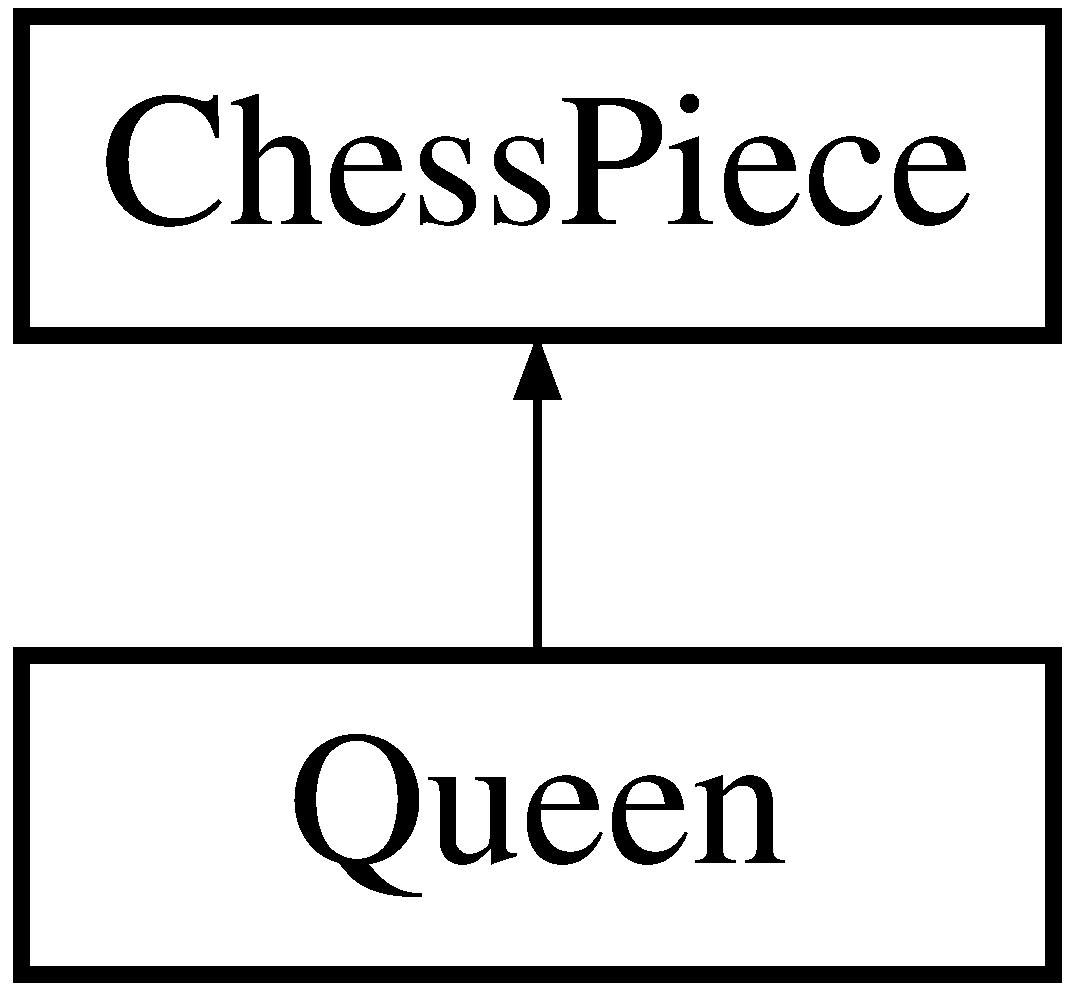
\includegraphics[height=2.000000cm]{class_queen}
\end{center}
\end{figure}
\subsection*{Public Member Functions}
\begin{DoxyCompactItemize}
\item 
\mbox{\Hypertarget{class_queen_acdfa2fb3cb38ecf2e178d7ef7db6bee7}\label{class_queen_acdfa2fb3cb38ecf2e178d7ef7db6bee7}} 
{\bfseries Queen} (\mbox{\hyperlink{class_board}{Board}} $\ast$board, \mbox{\hyperlink{class_square}{Square}} $\ast$location, Piece\+Color color)
\item 
\mbox{\Hypertarget{class_queen_aea5f53c17a06bb6524dc92b80f82d456}\label{class_queen_aea5f53c17a06bb6524dc92b80f82d456}} 
std\+::vector$<$ \mbox{\hyperlink{class_square}{Square}} $\ast$ $>$ {\bfseries get\+Available\+Squares} (bool consider\+Check)
\end{DoxyCompactItemize}
\subsection*{Additional Inherited Members}


The documentation for this class was generated from the following files\+:\begin{DoxyCompactItemize}
\item 
chesspieces/Queen.\+h\item 
chesspieces/Queen.\+cpp\end{DoxyCompactItemize}

\hypertarget{class_random_player}{}\section{Random\+Player Class Reference}
\label{class_random_player}\index{Random\+Player@{Random\+Player}}
Inheritance diagram for Random\+Player\+:\begin{figure}[H]
\begin{center}
\leavevmode
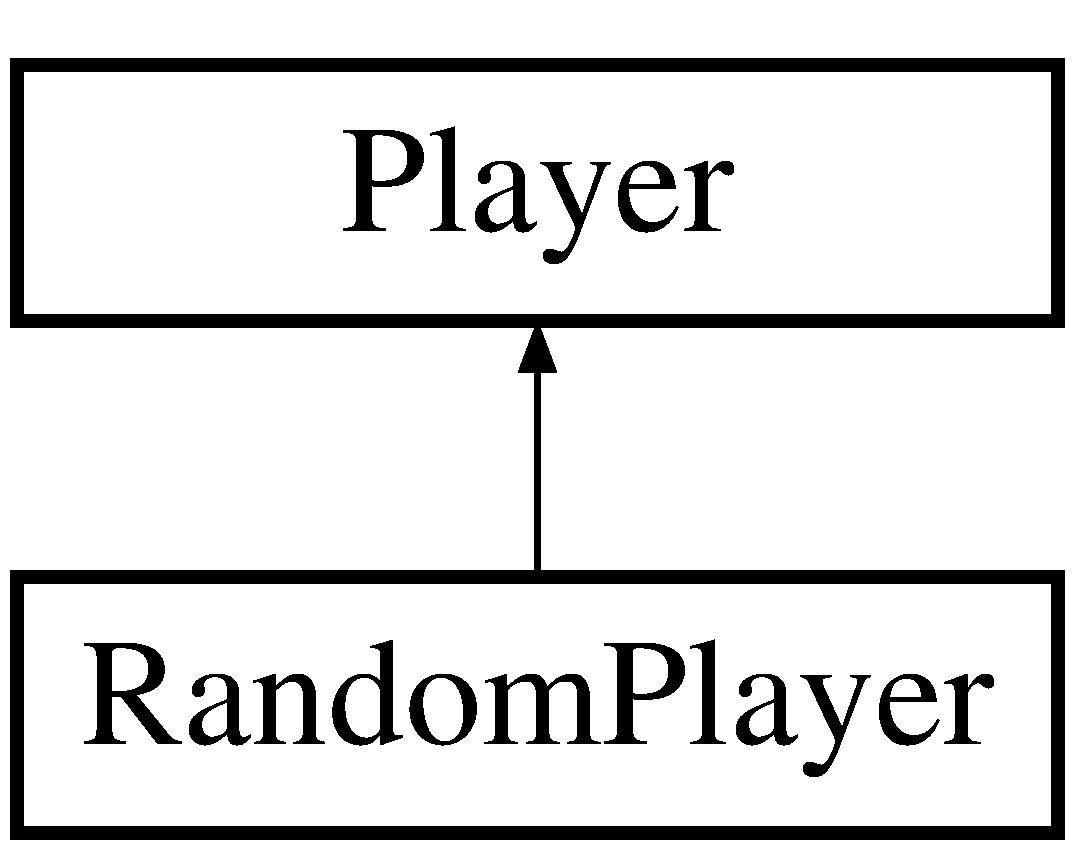
\includegraphics[height=2.000000cm]{class_random_player}
\end{center}
\end{figure}
\subsection*{Public Member Functions}
\begin{DoxyCompactItemize}
\item 
\mbox{\Hypertarget{class_random_player_a35590a358c0ef6dec72e7b33bfd98e36}\label{class_random_player_a35590a358c0ef6dec72e7b33bfd98e36}} 
{\bfseries Random\+Player} (Piece\+Color color)
\item 
\mbox{\Hypertarget{class_random_player_a12cb9e352db576ba61dad3dce938e4d8}\label{class_random_player_a12cb9e352db576ba61dad3dce938e4d8}} 
\mbox{\hyperlink{class_move}{Move}} $\ast$ {\bfseries get\+Next\+Move} (\mbox{\hyperlink{class_board}{Board}} $\ast$board)
\end{DoxyCompactItemize}
\subsection*{Additional Inherited Members}


The documentation for this class was generated from the following files\+:\begin{DoxyCompactItemize}
\item 
players/Random\+Player.\+h\item 
players/Random\+Player.\+cpp\end{DoxyCompactItemize}

\hypertarget{class_rook}{}\section{Rook Class Reference}
\label{class_rook}\index{Rook@{Rook}}
Inheritance diagram for Rook\+:\begin{figure}[H]
\begin{center}
\leavevmode
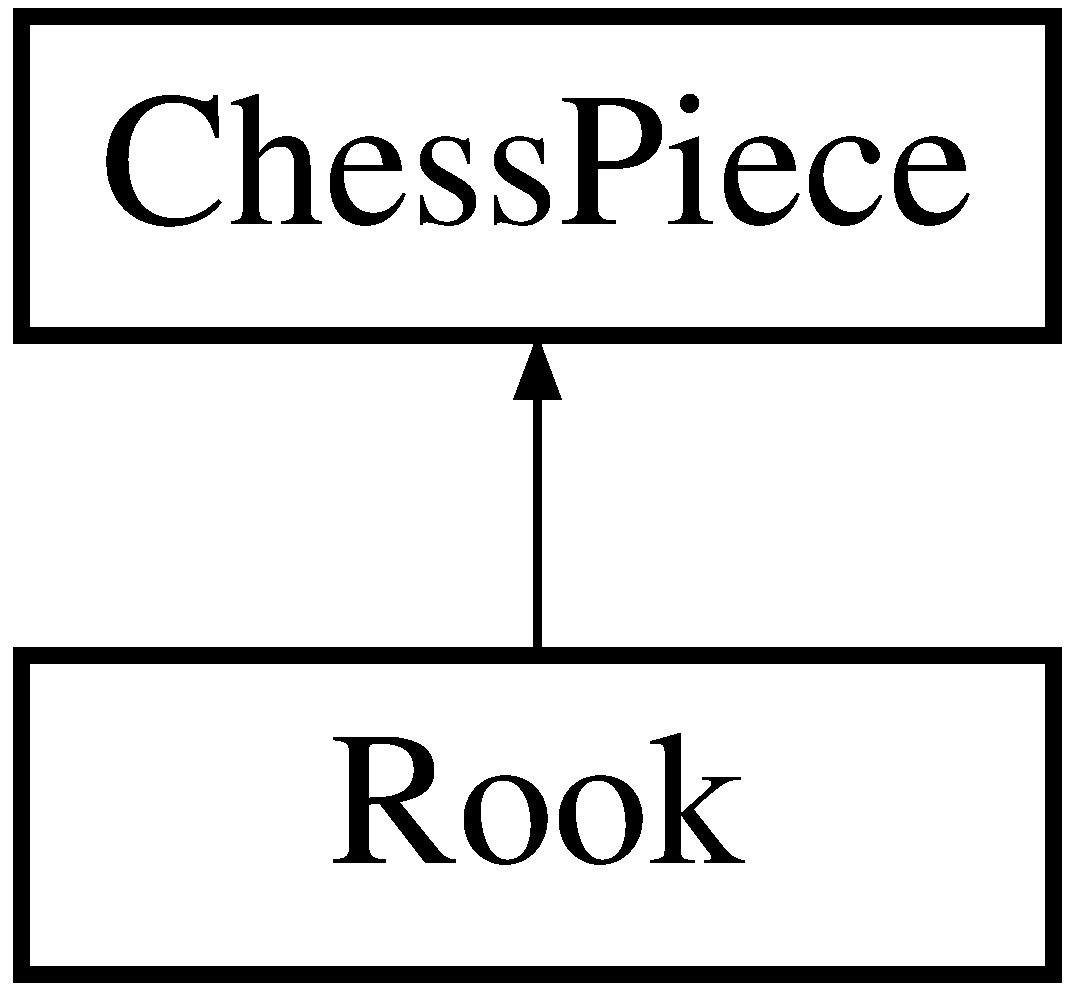
\includegraphics[height=2.000000cm]{class_rook}
\end{center}
\end{figure}
\subsection*{Public Member Functions}
\begin{DoxyCompactItemize}
\item 
\mbox{\Hypertarget{class_rook_a1c333105bdc3590b6d8379f39041e0a7}\label{class_rook_a1c333105bdc3590b6d8379f39041e0a7}} 
{\bfseries Rook} (\mbox{\hyperlink{class_board}{Board}} $\ast$board, \mbox{\hyperlink{class_square}{Square}} $\ast$location, Piece\+Color color)
\item 
\mbox{\Hypertarget{class_rook_a8078bb9a0382116d2f7ac76d39ecc5d3}\label{class_rook_a8078bb9a0382116d2f7ac76d39ecc5d3}} 
std\+::vector$<$ \mbox{\hyperlink{class_square}{Square}} $\ast$ $>$ {\bfseries get\+Available\+Squares} (bool consider\+Check)
\end{DoxyCompactItemize}
\subsection*{Additional Inherited Members}


The documentation for this class was generated from the following files\+:\begin{DoxyCompactItemize}
\item 
chesspieces/Rook.\+h\item 
chesspieces/Rook.\+cpp\end{DoxyCompactItemize}

\hypertarget{class_square}{}\section{Square Class Reference}
\label{class_square}\index{Square@{Square}}
\subsection*{Public Member Functions}
\begin{DoxyCompactItemize}
\item 
\mbox{\Hypertarget{class_square_a4bf015855b3e86e9385d3e026c0daafa}\label{class_square_a4bf015855b3e86e9385d3e026c0daafa}} 
{\bfseries Square} (int x, int y, int size, sf\+::\+Color color, sf\+::\+Vector2i coordinates)
\item 
\mbox{\Hypertarget{class_square_acdae90087b11bb963f79171ad9d5d5d1}\label{class_square_acdae90087b11bb963f79171ad9d5d5d1}} 
void {\bfseries draw\+Square} (sf\+::\+Render\+Window \&window)
\item 
\mbox{\Hypertarget{class_square_a662df4d28ccded0e1f37f0d9adac2620}\label{class_square_a662df4d28ccded0e1f37f0d9adac2620}} 
void {\bfseries set\+Selected} (bool selected)
\item 
\mbox{\Hypertarget{class_square_aca3e74cb55eab03037fc2e234b395bcf}\label{class_square_aca3e74cb55eab03037fc2e234b395bcf}} 
void {\bfseries set\+Focused} (bool focused)
\item 
\mbox{\Hypertarget{class_square_aa2eaed70acdcd0c0dd882732ff43ede3}\label{class_square_aa2eaed70acdcd0c0dd882732ff43ede3}} 
void {\bfseries set\+Chess\+Piece} (\mbox{\hyperlink{class_chess_piece}{Chess\+Piece}} $\ast$piece)
\end{DoxyCompactItemize}
\subsection*{Public Attributes}
\begin{DoxyCompactItemize}
\item 
\mbox{\Hypertarget{class_square_a1ec984a2cfe700db6fadaa258487f20f}\label{class_square_a1ec984a2cfe700db6fadaa258487f20f}} 
sf\+::\+Rectangle\+Shape {\bfseries rectangle}
\item 
\mbox{\Hypertarget{class_square_aa4d8f84fee8c9dcc2b8a24ba8856f18f}\label{class_square_aa4d8f84fee8c9dcc2b8a24ba8856f18f}} 
int {\bfseries posX}
\item 
\mbox{\Hypertarget{class_square_a7166f85a192ce8b683fb5b66353af3e7}\label{class_square_a7166f85a192ce8b683fb5b66353af3e7}} 
int {\bfseries posY}
\item 
\mbox{\Hypertarget{class_square_aae94641867db7a6b4d8558d0462f5f38}\label{class_square_aae94641867db7a6b4d8558d0462f5f38}} 
int {\bfseries size}
\item 
\mbox{\Hypertarget{class_square_a77552085b52b855d9d99a6c0d1f5a231}\label{class_square_a77552085b52b855d9d99a6c0d1f5a231}} 
sf\+::\+Color {\bfseries color}
\item 
\mbox{\Hypertarget{class_square_a88251e1e98ffa491e9aa661eb067776e}\label{class_square_a88251e1e98ffa491e9aa661eb067776e}} 
sf\+::\+Vector2i {\bfseries coordinates}
\item 
\mbox{\Hypertarget{class_square_acf73c354b081ef0ca2775e02d875ada0}\label{class_square_acf73c354b081ef0ca2775e02d875ada0}} 
bool {\bfseries is\+Selected} = false
\item 
\mbox{\Hypertarget{class_square_aa946d73869ef41e3a14d1888868c4650}\label{class_square_aa946d73869ef41e3a14d1888868c4650}} 
bool {\bfseries is\+Focused} = false
\item 
\mbox{\Hypertarget{class_square_a6ef91a5be2f1e3904973e75ee2115949}\label{class_square_a6ef91a5be2f1e3904973e75ee2115949}} 
bool {\bfseries is\+Checked} = false
\item 
\mbox{\Hypertarget{class_square_aa9199d2932f26c3ceee6d4101fb6196a}\label{class_square_aa9199d2932f26c3ceee6d4101fb6196a}} 
std\+::string {\bfseries name}
\item 
\mbox{\Hypertarget{class_square_ab67d2941bf8d4a0d2789053acb20e463}\label{class_square_ab67d2941bf8d4a0d2789053acb20e463}} 
\mbox{\hyperlink{class_chess_piece}{Chess\+Piece}} $\ast$ {\bfseries chess\+Piece} = N\+U\+LL
\end{DoxyCompactItemize}


The documentation for this class was generated from the following files\+:\begin{DoxyCompactItemize}
\item 
Square.\+h\item 
Square.\+cpp\end{DoxyCompactItemize}

%--- End generated contents ---

% Index
\backmatter
\newpage
\phantomsection
\clearemptydoublepage
\addcontentsline{toc}{chapter}{Index}
\printindex

\end{document}
